\documentclass{standalone}
\usepackage{tikz}
\usepackage{ctex,siunitx}
\usepackage{tkz-euclide}
\usepackage{amsmath}
\usetikzlibrary{patterns, calc}
\usetikzlibrary {decorations.pathmorphing, decorations.pathreplacing, decorations.shapes,}
\begin{document}
\small
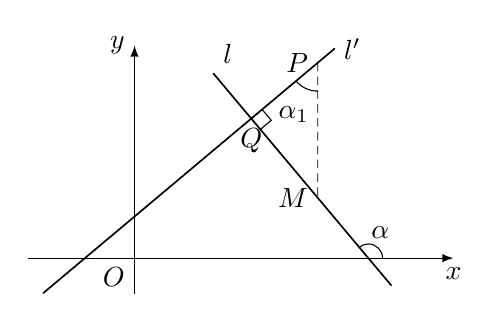
\begin{tikzpicture}[>=latex,scale=0.9]
  \begin{scope}
    \draw[thin,->](-1.5,0)--(4.5,0)node[below]{$x$};
    \draw[thin,->](0,-0.5)--(0,3.0)node[left]{$y$};
    \tkzDefPoints{3.3/0/B,-0.7/0/A,4/0/E,0/0/O}
    \tkzDefShiftPoint[B](130:2.0){C}
    \tkzDefPointBy[projection=onto B--C](A)\tkzGetPoint{Q}
    \tkzDefPointOnLine[pos=1.4](A,Q)\tkzGetPoint{P}
    \tkzDefPointOnLine[pos=3.5](B,C)\tkzGetPoint{D}
    \tkzDefPointBy[projection=onto A--B](P)\tkzGetPoint{N}
    \tkzInterLL(P,N)(B,C)\tkzGetPoint{M}
    \tkzDrawLine[semithick,add = 0.25 and 0.7](B,C)
    \tkzLabelLine[pos=1.7,above right](B,C){$l$}
    \tkzDrawLine[semithick,add = 0.25 and 0.5](A,Q)
    \tkzDrawSegments[densely dashed](P,M)
    \tkzLabelLine[pos=1.5,right](A,Q){$l'$}
    \tkzMarkAngle[size=0.2](E,B,Q)
    \tkzLabelAngle[pos=0.4](E,B,Q){$\alpha$}
    \tkzMarkAngle[size=0.4](Q,P,M)
    \tkzLabelAngle[pos=0.8](Q,P,M){$\alpha_1$}
    \tkzMarkRightAngle[size=0.2](P,Q,M)
    \tkzLabelPoints[below left](O)
    \tkzLabelPoints[below](Q)
    % \tkzLabelPoints[above left](P)
    \tkzLabelPoints[left](P,M)
  \end{scope}
\end{tikzpicture}
\end{document}